\subsection{Azienda ospitante}
RDS-NORDEST nasce nel 2007 da un gruppo di professionisti del mondo IT e della consulenza nell'area qualit� con esperienza decennale nel settore dei laboratori di prove e nella gestione della qualit� aziendale; l'azienda si � imposta rapidamente sul mercato grazie al forte know-how tecnico qualificandosi come azienda di riferimento nelle soluzioni software per la gestione dei laboratori di prove. Le principali soluzioni software offerte al mercato sono:
\begin{itemize}
\item \textbf{sistemi LIMS}: per la gestione dei laboratori di prove nelle configurazioni LIMS per i laboratori di controllo qualit� interni e LIMS per i laboratori conto terzi;
\item \textbf{quality management}: soluzioni software per il controllo qualit� interno;
\item \textbf{sales management}: suite di soluzioni software per la gestione delle vendite e dei rapporti con il canale GDO e Ho.Re.Ca.
\end{itemize}
Il personale aziendale � composto da tecnici laureati e non, ma tutti con profili professionali caratterizzati da esperienza pluriennale nel settore dei laboratori di prove; la value proposition che l'azienda offre consiste nell'automazione di processi e funzioni aziendali nel settore dei laboratori conto terzi e i clienti dell'azienda in tale settore sono tra i principali in Italia.

\subsection{Descrizione dello stage}
La pianificazione iniziale prevedeva come obiettivo minimo la realizzazione di uno schedulatore di attivit\`{a} ad hoc per laboratori che effettuano analisi chimiche, fisiche e merceologiche per conto terzi. L\textquoteright{}obiettivo di massimo era l\textquoteright{}integrazione dello schedulatore con un software in fase di sviluppo da parte dell\textquoteright{}azienda. Il tutto doveva essere preceduto dalla scelta della tecnologia da utilizzare per la realizzazione dello schedulatore.
A inizio stage la scelta della tecnologia \`{e} stata convenuta dall\textquoteright{}azienda. La soluzione consisteva nella modifica di un software opensource la cui funzionalit\`{a} era proprio quella di realizzare la pianificazione dei progetti utilizzando come strumento tecnico di pianificazione il diagramma di Gantt. Il software opensource pu\`{o} essere scaricato dalla piattaforma di SourceForge al seguente indirizzo: \url{http://sourceforge.net/projects/opproject/}.
Il software purtroppo \`{e} privo di documentazione, gli unici documenti reperibili sono i sorgenti dell\textquoteright{}applicativo scritti utilizzando il linguaggio Java. L\textquoteright{}adozione di questa soluzione \`{e} stata preceduta da uno studio di fattibilit\`{a} da parte dell\textquoteright{}azienda stessa, che a mio parere ha posto pi\`{u} attenzione ai pro della soluzione piuttosto che agli aspetti a sfavore nella scelta intrapresa. Infatti l\textquoteright{}applicativo \`{e} gi\`{a} sviluppato, ma essendo privo di documentazione, la sua manutenzione, adattativa e correttiva, nel caso in questione rischier\`{a} di far perdere all\textquoteright{}azienda molto tempo soprattutto perch\`{e} non \`{e} stato richiesto di integrare la parte di documentazione mancante all\textquoteright{}applicativo, quindi se l\textquoteright{}azienda dovesse apportare delle modifiche dovr\`{a} procedere prima con delle fasi di debugging al fine di comprendere le dinamiche del software per poi poter applicare le modifiche, il risultato finale \`{e} una pessima efficienza. Le ragioni di ci\`{o} sono testimoniate dall\textquoteright{}esperienza da me acquisita durante il progetto, per dare un\textquoteright{}idea quantitativa il software consiste in pi\`{u} di 1000 classi.
L\textquoteright{}azienda adottando la soluzione scelta ha immediatamente cambiato le milestones del mio progetto di stage. L\textquoteright{}obiettivo da raggiungere era proprio la realizzazione dello schedulatore ad hoc. Consultare la sezione di \nameref{sec:analisi} per i dettagli su quello che deve essere lo schedulatore ad hoc. La pianificazione quindi vede in aggiunta una fase di debugging inizialmente non prevista, e visti i tempi previsti per la durata dello stage, circa 300 ore \`{e} stata convenuta la rimozione dell\textquoteright{}obiettivo di massimo, da prevedere in un momento successivo, ma non nella baseline del mio progetto.

\newpage
\subsection{Pianificazione}

\begin{longtable}{>{\centering}p{5cm} >{\centering}m{17cm}}
La figura qui riportata presenta diagramma di Gantt vuole fornire una visione a preventivo del progetto a me commissionato, in particolare si tratta della pianificazione delle attivit\`{a} del progetto; tale piano di progetto � stato redatto in data 22/04/2013.
&
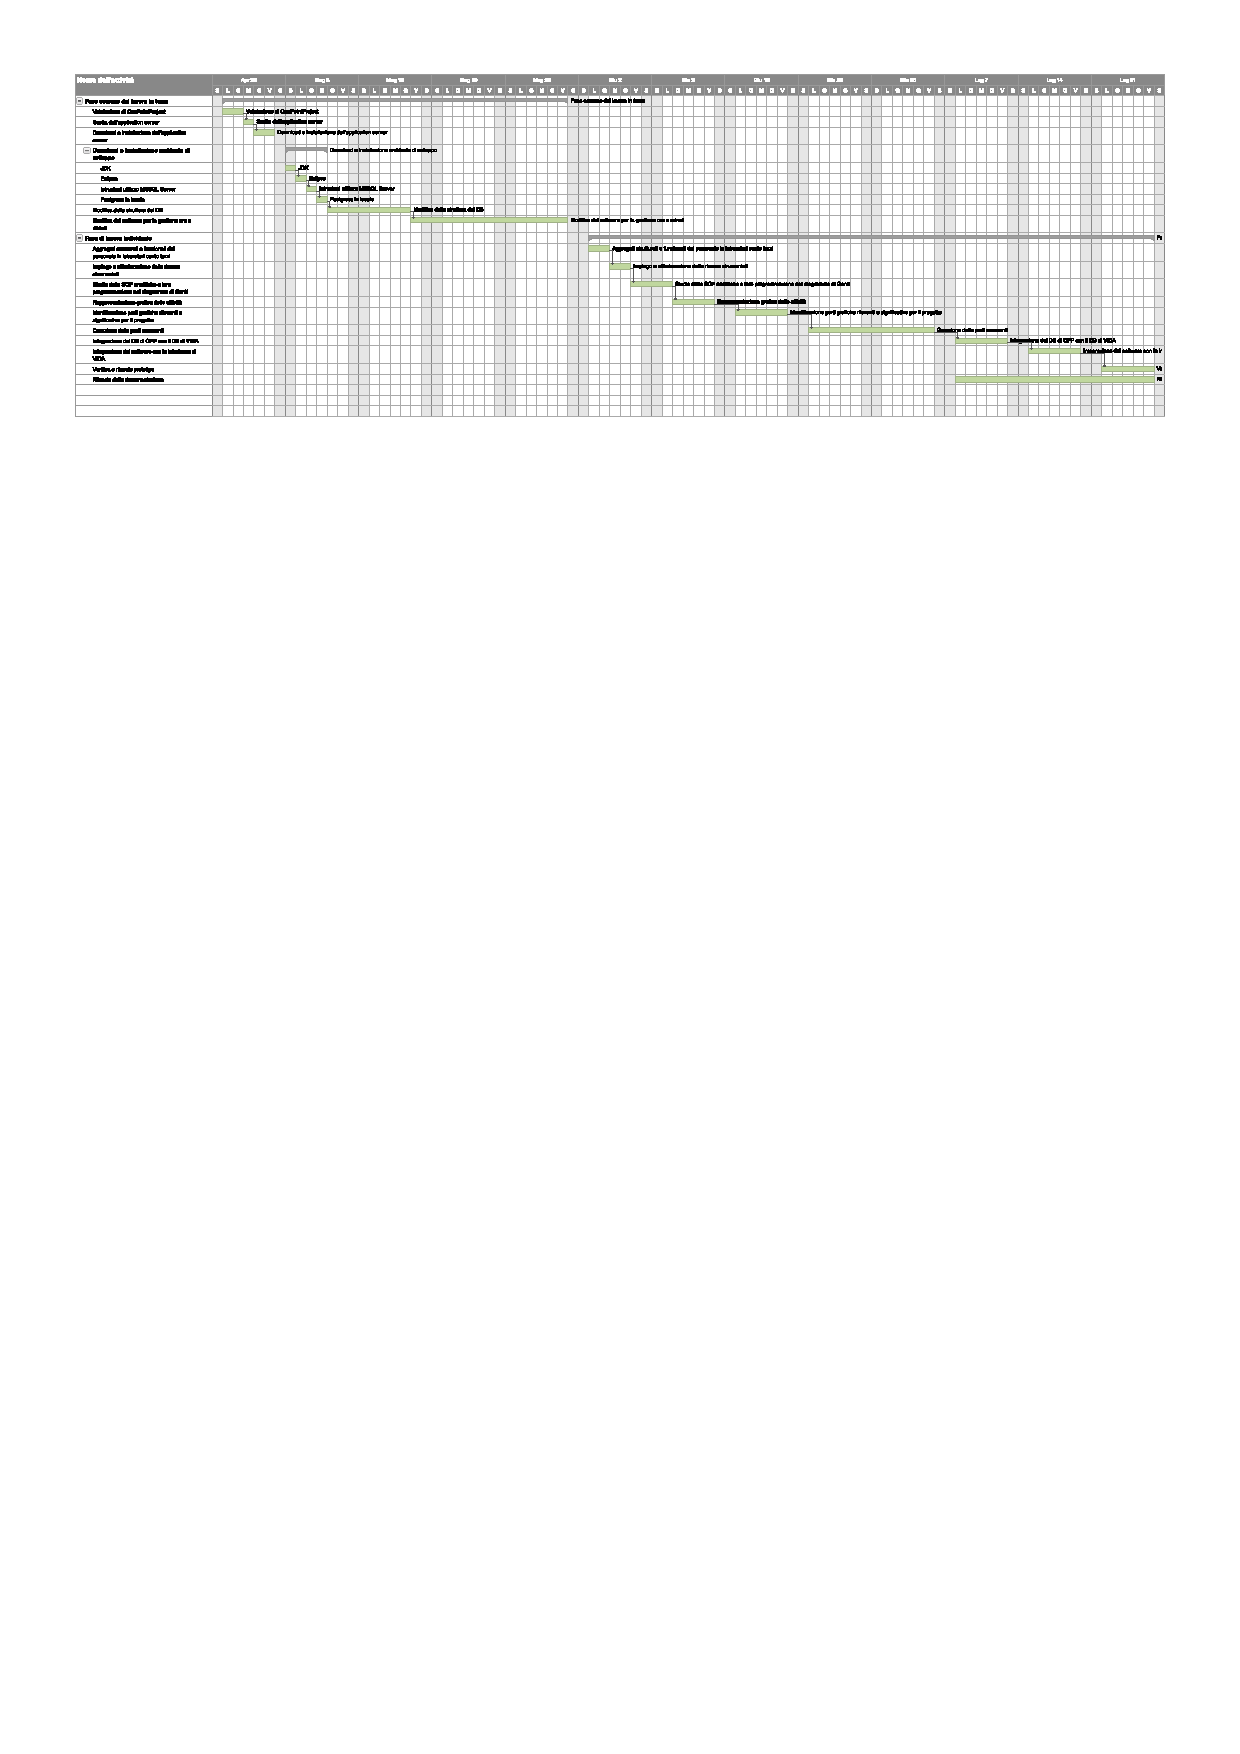
\includegraphics[width=1.5\textwidth,angle=90]{img/Preventivo1.pdf}
\end{longtable}

\newpage

\begin{longtable}{>{\centering}p{5cm} >{\centering}m{17cm}}
Il presente diagramma rappresenta l'aggiornamento del piano di progetto in relazione alla scelte implementative dell\textquoteright{}azienda che ha quindi parzialmente modificato i requisiti del progetto.
&
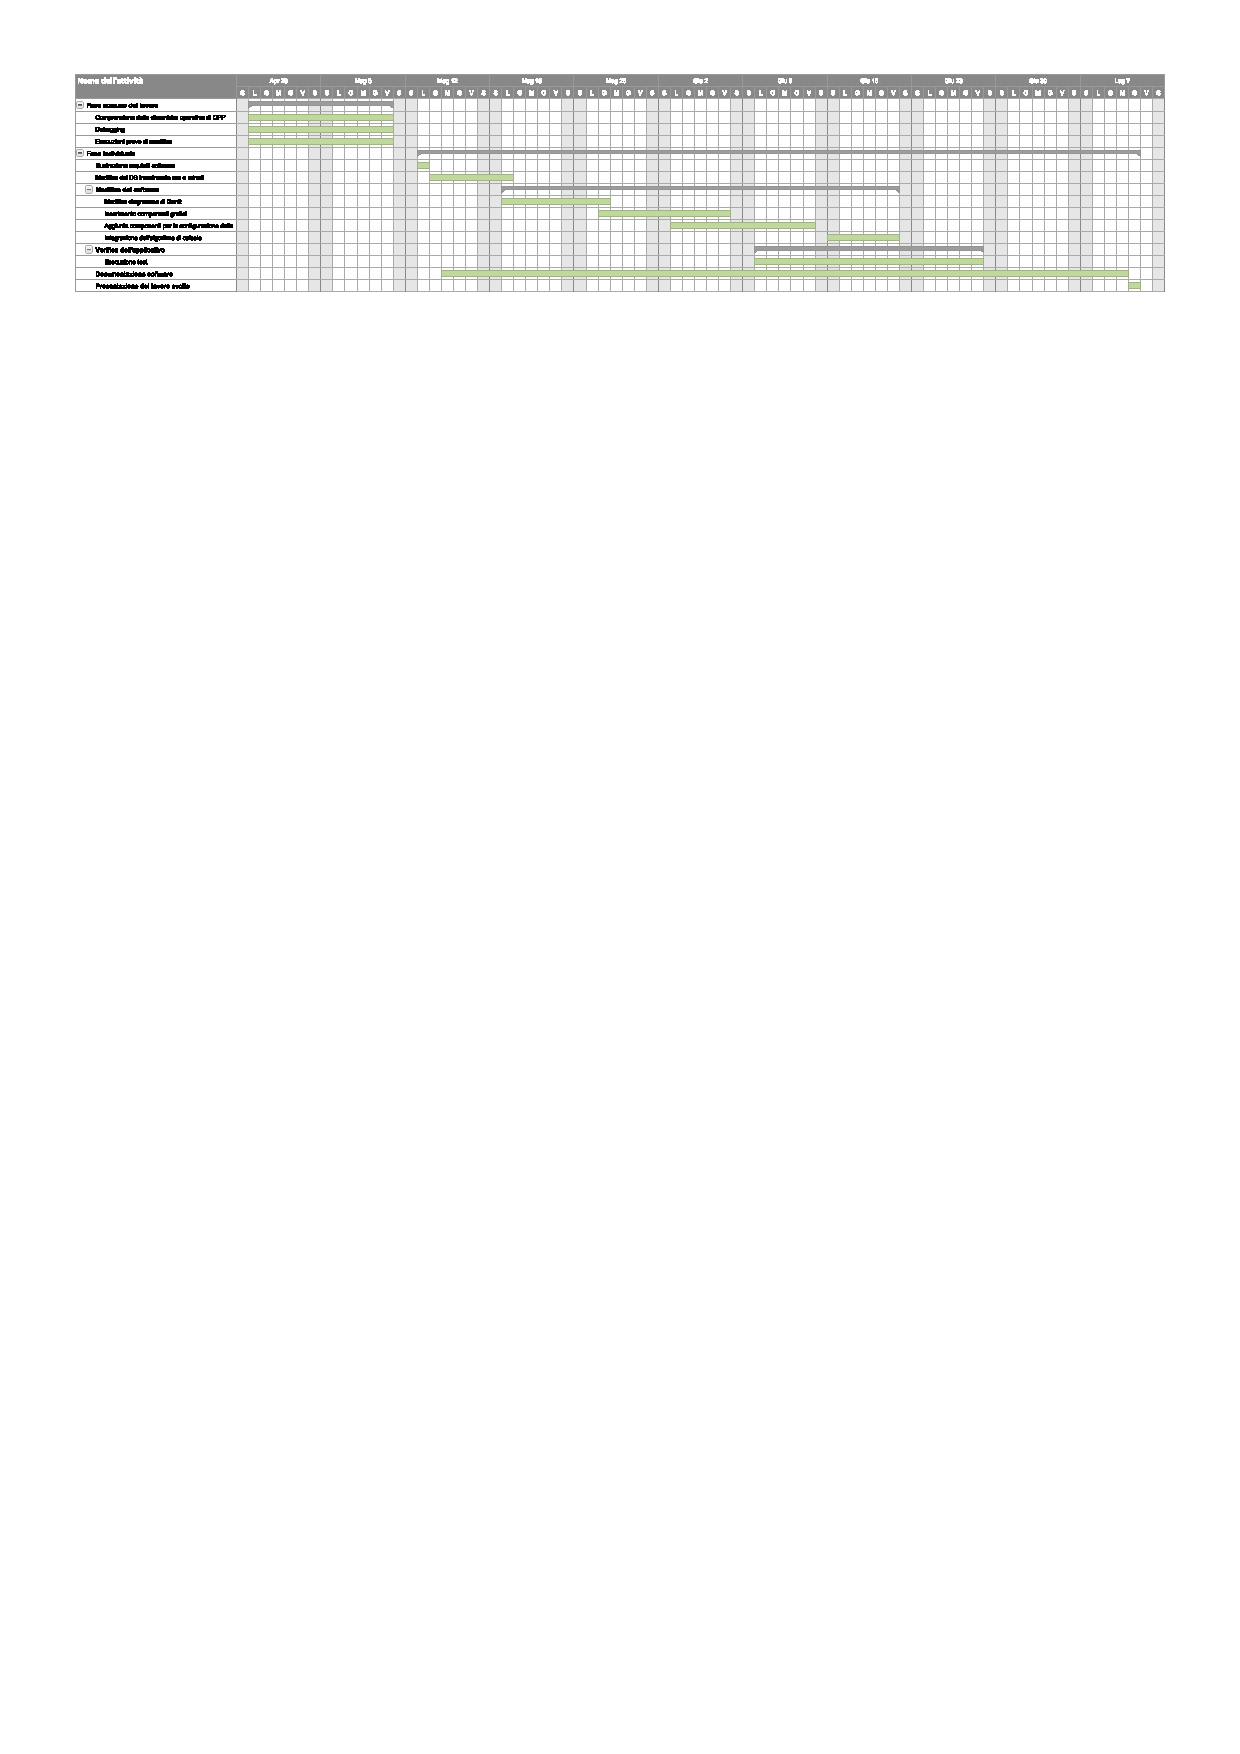
\includegraphics[width=1.6\textwidth,angle=90]{img/Preventivo2.pdf}
\end{longtable}

\newpage

\begin{longtable}{>{\centering}p{5cm} >{\centering}m{17cm}}
Un diagramma di Gantt a preventivo, come quelli presentati, si dimostra utile per capire quali sono le dipendenze delle attivit\`{a}, la loro durata (meglio con un diagramma di Pert), le scadenze. I diagrammi di Gantt a consuntivo possono essere utilizzati come strumento di misurazione dell\textquoteright{}abilit\`{a} di un project Manager nella pianificazione dei progetti, tale strumenti quindi possono essere utilizzati al fine di mirare al miglioramento continuo in logica PDCA. Il seguente diagramma rappresenta il consuntivo delle attivit� realizzate.
&
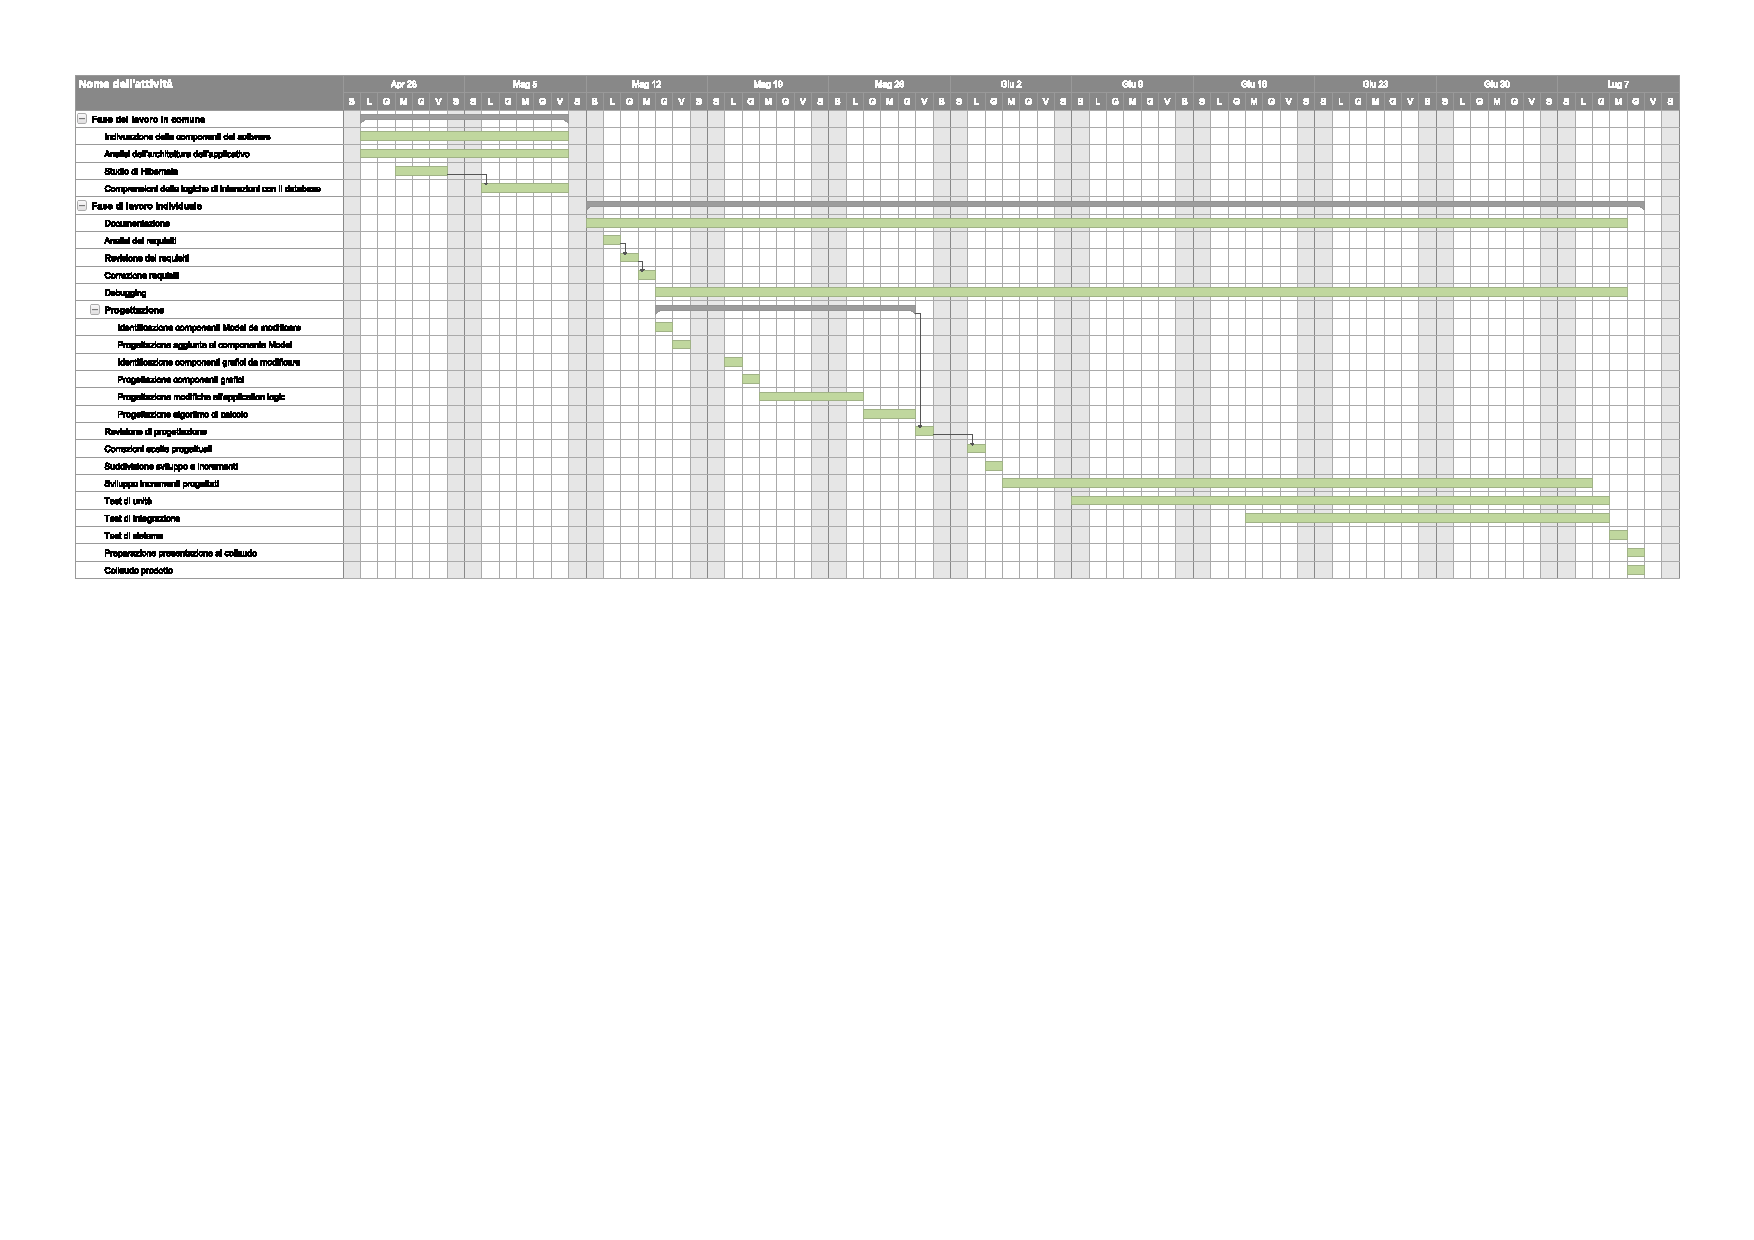
\includegraphics[width=1.6\textwidth,angle=90]{img/Consuntivo.pdf}
\end{longtable}

\subsubsection{Ciclo di vita}
Il modello di ciclo di vita dell\textquoteright{}azienda rientra tra le metodologie agili. L\textquoteright{}azienda settimanalmente produce il cosidetto \textit{``sprint planning\textquoteright{}\textquoteright{}} ovvero pianifica le attivit\`{a} da svolgere nella settimana successiva. A questa fase si susseguono le attivit\`{a} di verifica pianificate, sia relative allo stato di avanzamento del prodotto sia relative alla qualit\`{a} del prodotto. In relazione al ciclo di vita adottato dall\textquoteright{}azienda ovviamente con gli stagisti ha adottato lo stesso approcio fornendo sul mio progetto revisioni eseguite con una frequenza pari a 2 settimane. Il progetto da me svolto per le caratteristiche presentate si \`{e} concordato con il modello dell\textquoteright{}azienda per quanto riguarda i processi di revisione e di comunicazione; tuttavia \`{e} stato indispensabile adottare per il progetto un ciclo di vita incrementale, nello specifico sono stati pianificati e poi mantenuti \textit{4 incrementi}. La natura del ciclo adottata \`{e} stata incrementale proprio a causa del modello adottato dall\textquoteright{}azienda. Infatti il dettaglio dei requisiti del progetto, sono emersi non dall\textquoteright{}inizio ma durante lo stage e quindi durante il ciclo di vita stesso. Il progetto quindi ha prodotto un software la cui vita \`{e} stata animata da baseline successive.